\subsection{Tarjan package}

In questa sezione descriveremo il package \textbf{tarjan}.

Questo package non contiene molte astrazioni ma si limita a definire
un contratto fondamentale per implementare la visita \emph{DFS} e
l'algoritmo di Tarjan.

\subsubsection*{Supplied Abstractions}

Le astrazioni fornite da questo package sono le seguenti:
\begin{itemize}
\item definire il contratto nel quale vengono stabiliti gli eventi
  salienti che avvengono durante la visita \emph{DFS} del
  grafo. Questi eventi vengono codificati come messaggi che possono
  essere inviati ad un implementatore del contratto, in modo da
  notificare che la ricerca si trova in un determinato stato. Questo
  permette non solo di codificare la visita, bensi adattarne il
  comportamento secondo le proprie esigenze e creare delle varianti
  della stessa (come in realt\`a lo \`e lo stesso algoritmo di
  Tarjan).
\item fornire due implementatori del contratto descritto nel punto
  precedente, uno che permette di costruire un grafo (o, per esser
  pi\`u precisi, un albero) che rappresenta la visita \emph{DFS},
  costituito dal sottoinsieme di archi visitati; l'altro costruisce un
  grafo che \`e la minimizzazione di un grafo iniziale al quale si
  applica l'algoritmo di Tarjan. I nodi del grafo risultate sono le
  componenti fortemente connesse identificate dall'algoritmo.
\end{itemize}

\subsubsection*{Class diagram}
Il diagramma rappresentato in figura \ref{fig:tarjan-package-classes}
rappresenta i concetti implementati in questo package. Procediamo con
ordine nel descrivere le idee principali catturate da ogni classe:

\begin{figure}
  \centering
  % 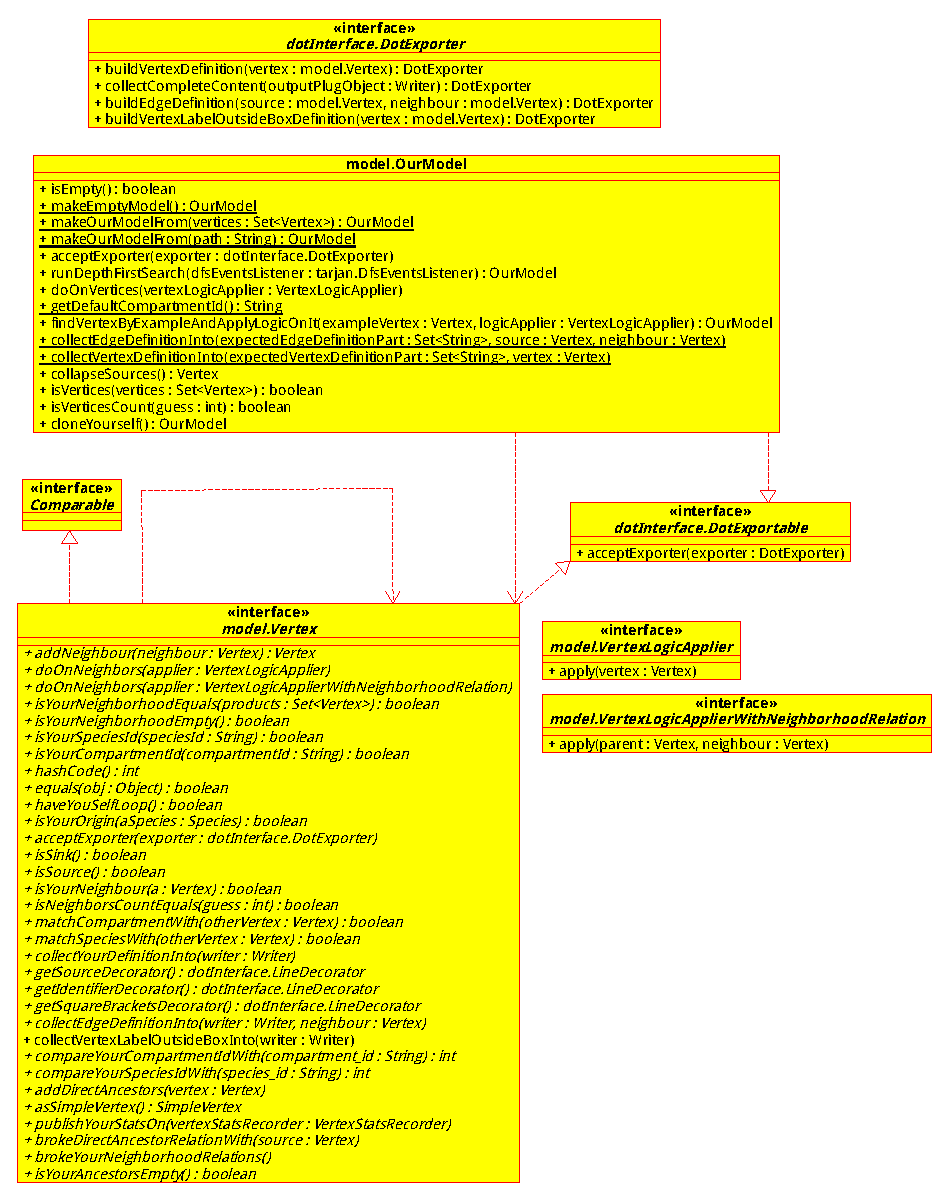
\includegraphics{packages/vertex-interface-class-diagram.eps} 
  \caption{Tarjan package's classes}
  \label{fig:tarjan-package-classes}
\end{figure}

\begin{paragraph}{DfsEventsListener}
Questo contratto permette di astrarre gli stati che si possono
incontrare durante una visita \emph{DFS} in modo da permettere non
solo l'implementazione della visita stessa, bensi anche di sue
varianti. Riporto sotto la sua definizione direttamente dal relativo
file sorgente:

\begin{lstlisting}
package tarjan; 
public interface DfsEventsListener {

  void searchCompleted(Map<Vertex, ExploreStatedWrapperVertex> map);
  void postVisit(Vertex v);
  void preVisit(Vertex v);
  void searchStarted(Map<Vertex, ExploreStatedWrapperVertex> map);
  void newVertexExplored(Vertex explorationCauseVertex, Vertex
    vertex);
  void fillCollectedVertices(Set<Vertex> vertices);
  void alreadyKnownVertex(Vertex vertex);
  }
\end{lstlisting}
Il motore che utilizza questa interfaccia \`e la classe
\emph{OurModel}. Aver definito questo contratto ci ha permesso di dare
una implementazione molto object-oriented, che differisce nello stile
rispetto ad una implementazione pi\`u comune in un linguaggio
procedurale. Credo sia interessante vederla, per cui mi dilungher\`o
in questi paragrafi nella sua descrizione. L'\emph{entry-point} della
computazione \`e il seguente metodo definito nella classe
\emph{OurModel}:
\begin{lstlisting}
  public OurModel runDepthFirstSearch(DfsEventsListener
  dfsEventsListener) { 
    final Map<Vertex, ExploreStatedWrapperVertex> map = makeDfsVertexMetadataMap();
    dfsEventsListener.searchStarted(map);
    for (Entry<Vertex, ExploreStatedWrapperVertex> entry : map.entrySet()) {
      entry.getValue().ifNotExplored(dfsEventsListener,	new
      ExploreStateWrapperVertexMapper() 
      {
        @Override
	public ExploreStatedWrapperVertex map(Vertex vertex) {
          return map.get(vertex);
	}
      });
    }
    dfsEventsListener.searchCompleted(map);
    return this;
  }
\end{lstlisting}
Questo metodo incapsula l'algoritmo della ricerca \emph{DFS}, usando
il listener passato come argomento, per notificare cosa st\`a
accadendo durante la ricerca. Come si nota, mancano alcuni pezzi per
avere una \emph{DFS} corretta: questi sono stati incapsulati nella
classe \emph{ExploreStateWrapperVertex} per avere un sistema pi\`u
object-oriented, rispetto a codificare tutto nel metodo sopra
riportato. La responsabilit\`a di questa nuova classe \`e quella di
associare ad ogni vertice l'informazione se questo \`e gia stato
visitato oppure no durante la visita. Inoltre, possiamo chiedere ad
oggetti istanze di questa classe, di esplorare il loro vicinato se non
sono gia stati esplorati, inviando il messaggio \emph{ifNotExplored}
che riporto:
\begin{lstlisting}
public class ExploredStateWrapperVertex...
  public ExploreStatedWrapperVertex ifNotExplored(
  final DfsEventsListener dfsEventsListener,
  Vertex explorationCauseVertex,
  final ExploreStateWrapperVertexMapper mapper) {
    final Vertex vertex = getWrappedVertex();
    if (isExplored() == false) {
      toggle();
      if (explorationCauseVertex != null) {
        dfsEventsListener.newVertexExplored(explorationCauseVertex,vertex);
      }
      dfsEventsListener.preVisit(vertex);
      vertex.doOnNeighbors(new VertexLogicApplierWithNeighborhoodRelation() {
        @Override
        public void apply(Vertex parent, Vertex neighbour) {
          if ((parent == vertex) == false) {
            throw new RuntimeException("Semantic error");
          }
          mapper.map(neighbour).ifNotExplored(dfsEventsListener,parent, mapper);
        }
      });
      dfsEventsListener.postVisit(vertex);
    } else {
      dfsEventsListener.alreadyKnownVertex(vertex);
    }
    return this;
}
\end{lstlisting}
Questo \`e il blocco mancante nel metodo precedente e che
effettivamente caratterizza la ricerca \emph{DFS} (linea 19). Nel
metodo sopra riportato inoltre si nota che \`e stato molto semplice
implementare questa parte, in quanto, data la natura ricorsiva
dell'implementazione, non dobbiamo far altro che invocare lo stesso
metodo su tutti i vertici del vicinato. Sar\`a il loro stato che
propagher\`a ancora il messaggio al rispettivo vicinato oppure, nel
caso il vertice sia gi\`a stato visitato, verr\`a segnalato al
listener questo evento inviando il messaggio
\emph{alreadyKnownVertex}. Una ultima osservazione deve essere fatta
riguardo agli eventi notificati: i listener concreti non per forza
devono definire della logica per ogni evento, in quanto ognuno di
questi viene creato per implementare una specifica variante e non
necessariamente ogni evento \`e richiesto per terminare quanto
desiderato.
\end{paragraph}

\begin{paragraph}{DfsEventsListenerTreeBuilder}
  Questo listener permette di associare ad ogni vertice delle
  informazioni per costruire l'albero \emph{DFS} che rappresenta la
  ricerca. In particolare si mantiene una coppia di istanti $(t_{in},
  t_{out})$ dove $t_{in}$ rappresenta l'istante in cui il vertice
  viene esplorato, $t_{out}$ rappresenta l'istante in cui si \`e
  finito di esplorare il rispettivo vicinato e la chiamata ricorsiva
  termina per tale vertice.

  Inoltre, nella gestione dell'evento \emph{newVertexExplored}, si
  costruisce la nuova relazione di vicinato, includendo solo quegli
  archi che hanno portato all'esporazione di nuovi vertici e che
  caratterizzano l'albero \emph{DFS} risultante.

  Riprendendo l'osservazione fatta al termine del paragrafo
  precedente, questo listener non ha bisogno di definire nessuna
  logica per l'evento \emph{alreadyKnownVertex}.
\end{paragraph}

\begin{paragraph}{TarjanEventsListenerTreeBuilder}
  Questo listener implementa l'algoritmo di Tarjan e codifica il
  comportamento per produrre un grafo i cui nodi sono le componenti
  fortemente connesse che si possono individuare nel grafo di
  input. 

  Questo grafo contiene come vertici degli oggetti che hanno
  comportamento specifico relativo alle componenti connesse, per cui,
  nelle successive computazioni, sar\`a possibile usare il grafo in
  modo astratto, inviando messaggi polimorfi che produrranno il
  comportamento desiderato (ad esempio la rappresentazione
  dell'etichetta nel documento grafico sar\`a diversa rispetto a
  quella che si pu\`o ottenere dopo una visita \emph{DFS}).
\end{paragraph}



